\documentclass[MiniProjectMain]{subfiles}
\begin{document}

\chapter{Theory}

\section{Cyclic syndrome decoding}
The syndrome of a cyclic code can be calculated efficiently using a sequential division circuit (See Figure \ref{fig:CyclicSyndromeDecoder}), based on the generator polynomial.
This is done by shifting the entire received vector into the division circuit.

The syndrome of the received vector is now readable in the delay line of the division circuit.
If the circuit is then shifted further, with no input but except any correction bits, the next syndrome is readable in the delay line of the division circuit.

This is employed in the Meggitt decoder to continuously check for errors in the received vector.

\begin{figure}[H]
\begin{center}
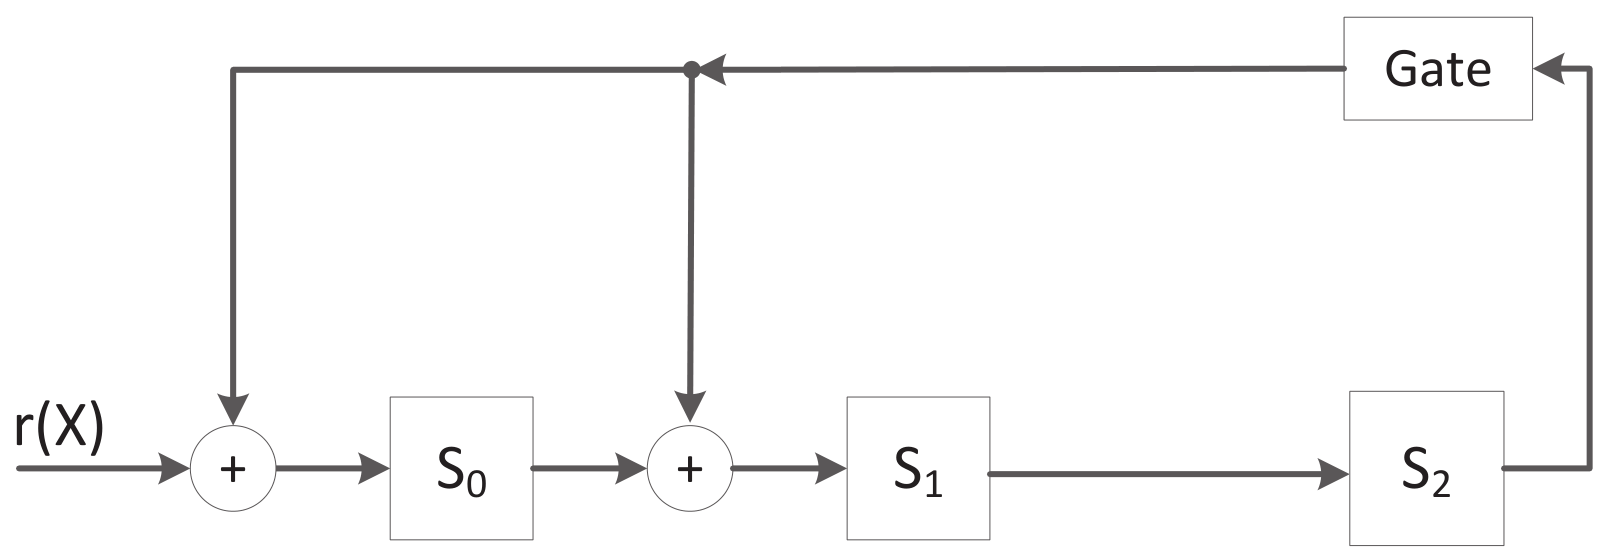
\includegraphics[width = \textwidth]{CyclicSyndromeDecoder}
\caption{Sequential division circuit for generator polynomial: 
$g(X) = 1 + X + X^3$
}
\label{fig:CyclicSyndromeDecoder}
\end{center}
\end{figure}

\newpage
\section{Meggitt decoding}

\subsection{The Meggitt decoding circuit}
In figure \ref{fig:CyclicDecoder} the circuit of the Meggitt decoder is presented.


\begin{figure}[H]
\begin{center}
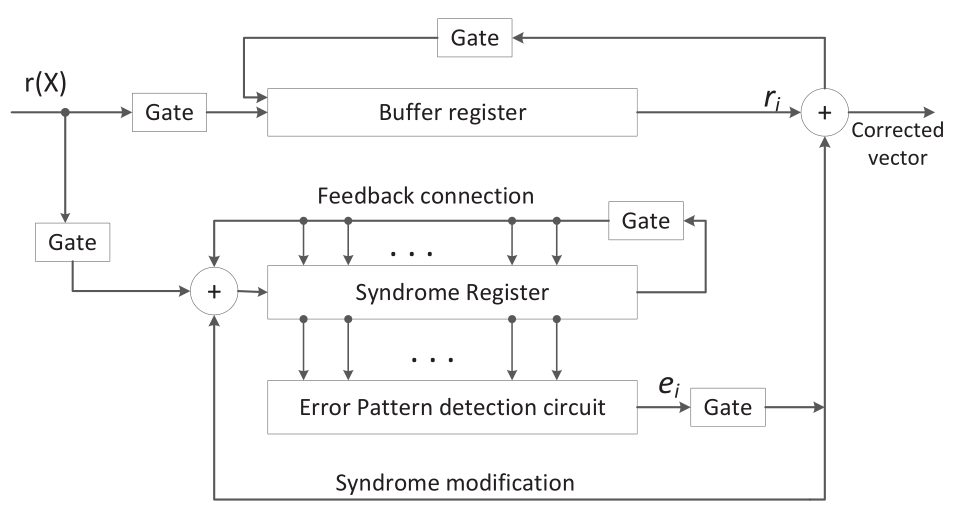
\includegraphics[width = \textwidth]{CyclicDecoder}
\caption{Meggitt decoder circuit}
\label{fig:CyclicDecoder}
\end{center}
\end{figure}

The Meggitt decoder consist of:
\begin{itemize}
\item
A receive buffer \textit{r(x)}

\item
A Buffer register

\item
A division circuit with a Syndrome register

\item
An Error Pattern detection circuit

	\begin{itemize}
	\item This circuit normally consist of combinational logic for single error detection, and table lookup in multi error detection.
	\end{itemize}

\item
A Code register containing the corrected vector.

\end{itemize}

\subsection{The Meggitt decoding algorithm}

\begin{enumerate}

\item
Shift the entire received vector into the Buffer register and Syndrome register simultaneously.

\item
Compare Syndrome register with all syndromes for errors in the last position of the codeword.
\label{step:compare}

	\begin{itemize}
	\item[--]
	If the syndrome matches output a '1' from the Error detection circuit.
	
	\item[--]
	Else output a '0' from the Error detection circuit.
	\end{itemize}
	
\item
Shift the Buffer and Syndrome register ahead once.

	\begin{itemize}
	\item[--]
	The corrected symbol is shifted into the Code register
	\item[--]
	The Syndrome feedback is also corrected
	\end{itemize}
	
\item
If the entire codeword have not yet been shifted out of the Buffer register, proceed from step \ref{step:compare}. 
Else proceed to step \ref{step:tag}.

\item
Check validity of corrected codeword.
\label{step:tag}
	
	\begin{itemize}
	\item[--]
	If the Syndrome register zero vector, then the corrected codeword is a valid codeword.
	The codeword can still have been affected by a undetectable error pattern.
	
	\item[--]
	Else: An uncorrectable error has been detected.
	
	\end{itemize}





\end{enumerate}

\end{document}